To investigate how well the the archetypes, which perform the suggested strategies, seperate data, the predictive power of archetypes as a target variable in a supervised learning paradigm is investigated. The prediction accuracy is compared to that of plain BFTs as well as PCs of QIs, of which there are also six. Data from the SensibleDTU experiment is used. As is shown in Section \ref{subsubsec:analysisAndData}, different strategies tended to be adopted by people in different age groups, and since the population in the SensibleDTU dataset is strictly composed of students, conclusions must be drawn with a degree of respect for this bias. Details of the analysis are are discussed in Section \ref{subsec:classification}.

Optimized prediction models are trained on 38 indicators to predict low, medium or high distance to each of the archetypes. Figure \ref{fig:classification_results_CA} visualizes the accuracies, and explains high-level aspect of the applied procedure. It is compared to prediction accuracies for Big Five traits (Figure \ref{fig:classification_results_BFT}) and PCs of Big Five Inventory QIs (Figure \ref{fig:classification_results_PCA}) using the same approach. There are discovered to be six PCs in QI-space as shown in Figure \ref{fig:significantPCs}. The remainder of this section presents the results.

\textbf{Distances to archetypes are predicted with highest accuracies}.
Average prediction accuracies above baseline (AB) reported in Figure \ref{fig:classification_results_CA}, \ref{fig:classification_results_BFT} and \ref{fig:classification_results_PCA} are 5.8\%, 2.4\ and 4.1\%, respectively. As such PCs can be predicted better than BFTs and distance from archetypes can be predicted better than PCs. Prediction accuracy compares to, but is not better than what has already been reported for prediction of BFTs in previous studies\mcite{monsted2016phone, de2013predicting}. This may be upsetting in terms of the predictive promise of the behavioral indicators computed using the extended version of the bandicoot software (see Section \ref{subsubsec:featureEngineering}), but on the other hand it also shows that archetypes do split the data better.

\begin{figure}[b]
	\centering
	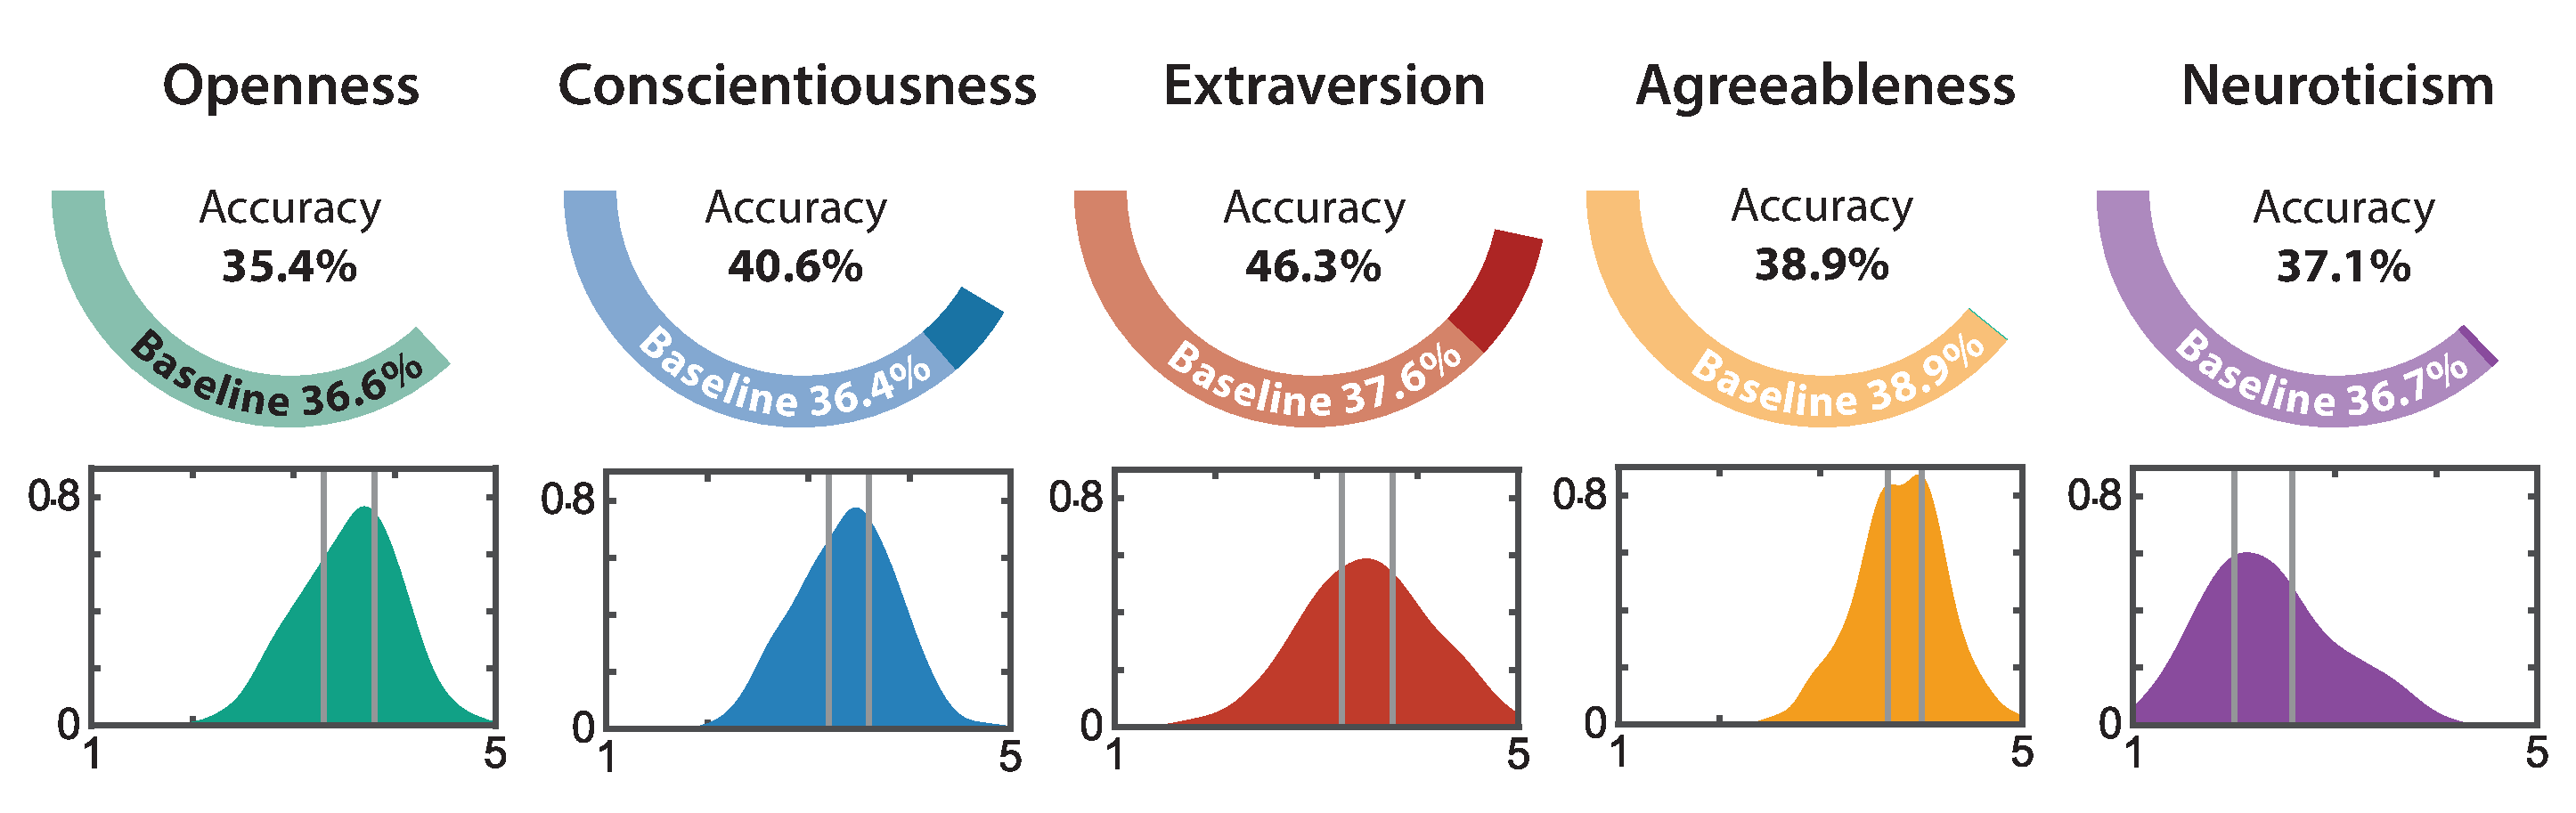
\includegraphics[width=\textwidth]{figures/classification_results}
	\caption{\label{fig:classification_results_BFT} Three-class classification accuracy of BFTs predicted from behavioral indicators. Only C and E can be predicted Same procedure as described in Figure \ref{fig:classification_results_CA}.}
\end{figure}

\textbf{Archetypes are predicted better than their parts}.
In the current approach only \CON and \EXT can be predicted well. Considering the \achiever archetype, prediction accuracy is 6.8\% AB, yet out of these two BTFs this archetype only varies on \CON which has prediction accuracy 4.2\% AB. It is unclear what accounts for this difference, and further analysis is requires to understand it. 

\begin{figure}[h!]
	\centering
	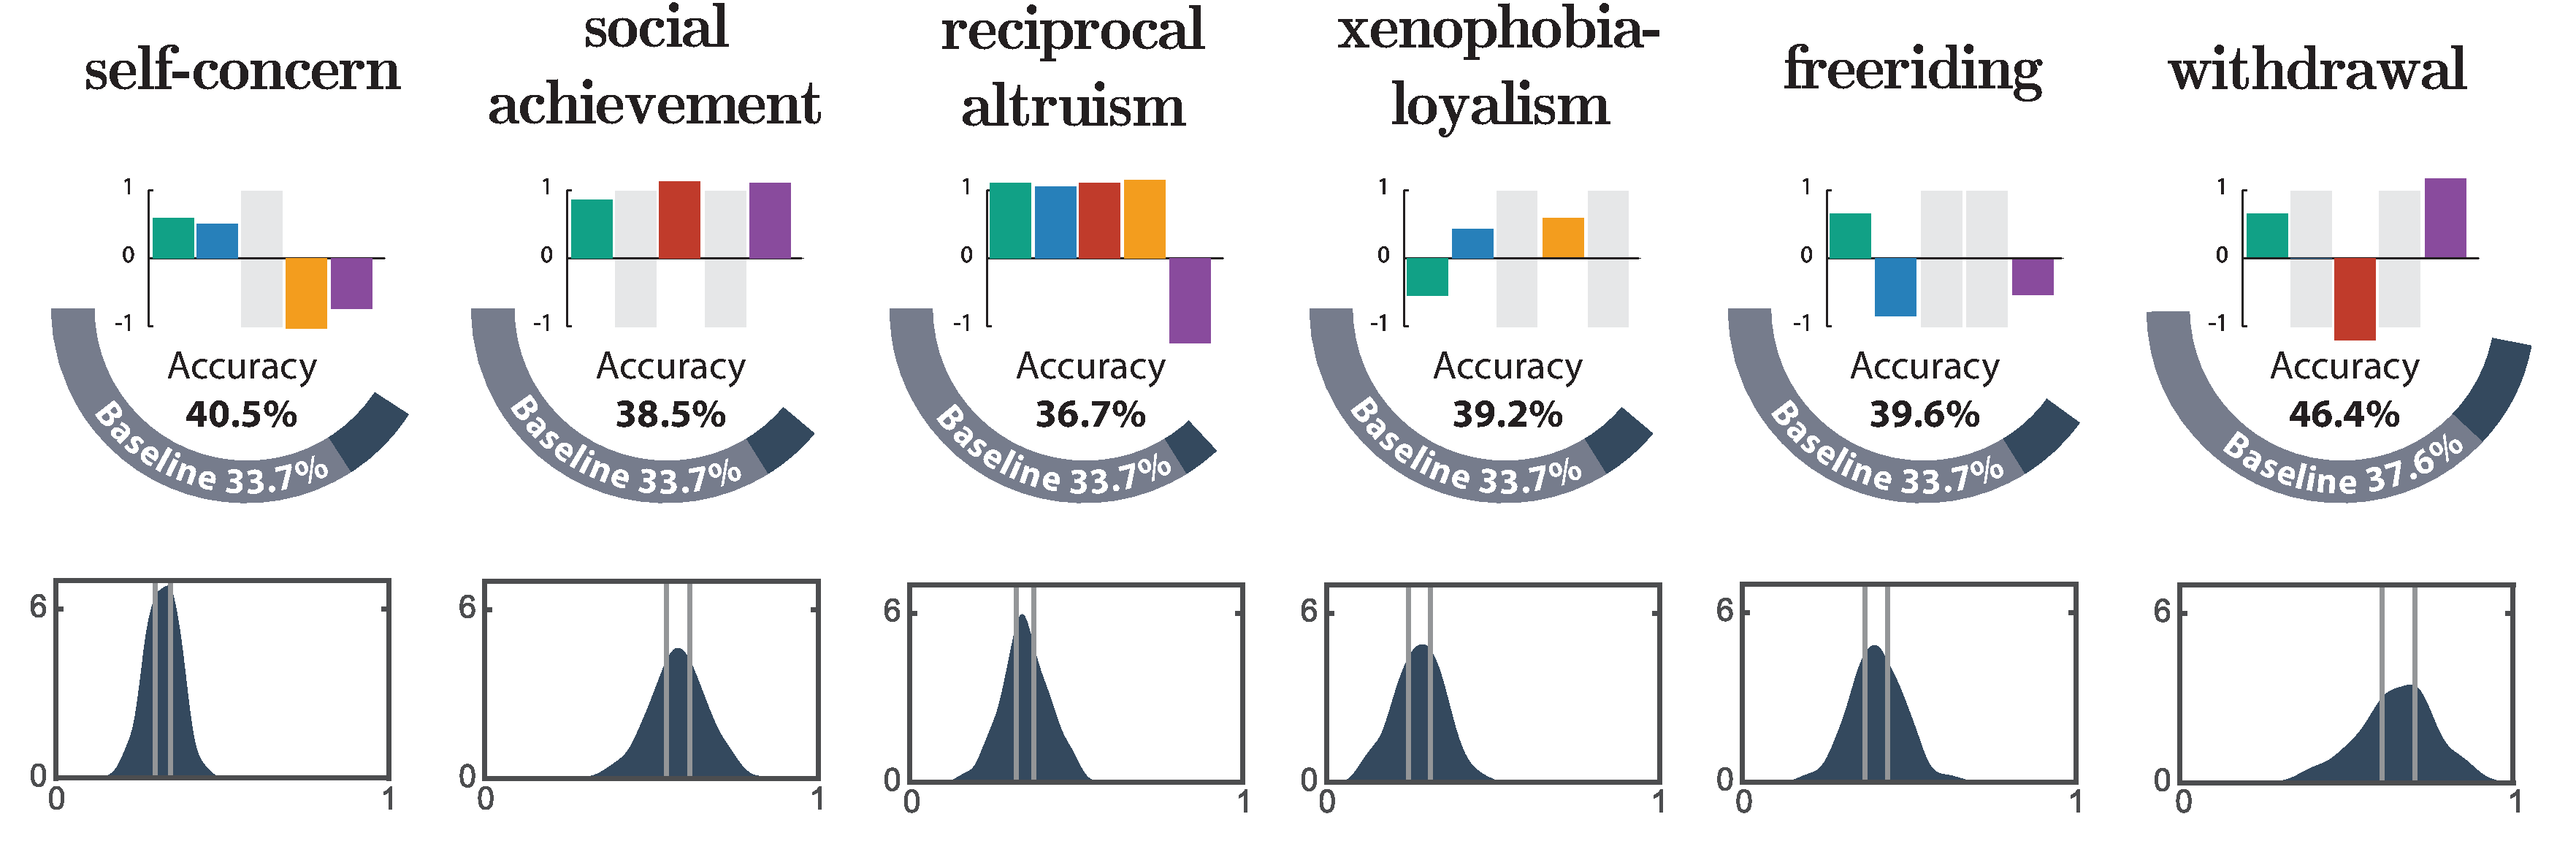
\includegraphics[width=\textwidth]{figures/classification_results_CA}
	\caption{\label{fig:classification_results_CA} Three-class classification accuracy of archetypes predicted from behavioral indicators. Samples are split into three semi-balanced classes based on their target values (low, medium, high). Sample distributions are shown as KDE plots below each score diagram, and vertical lines show decision boundaries. Reported accuracies are averages over 100 shuffled stratified cross validation folds of parameter optimized random forest models (random search and grid search), with standard errors in the range of .2 to .5 percent. Baselines are calculated as the of size of the largest class divided by number of samples. The bar diagrams show how each component/archetype is interpreted in terms of BFTs, where height is the normalized archetype position in BF space and non-consensus dimensions are shown in grey.}
\end{figure}

\begin{figure}[h!]
	\centering
	\begin{minipage}[l]{0.5\textwidth}
		\flushleft
		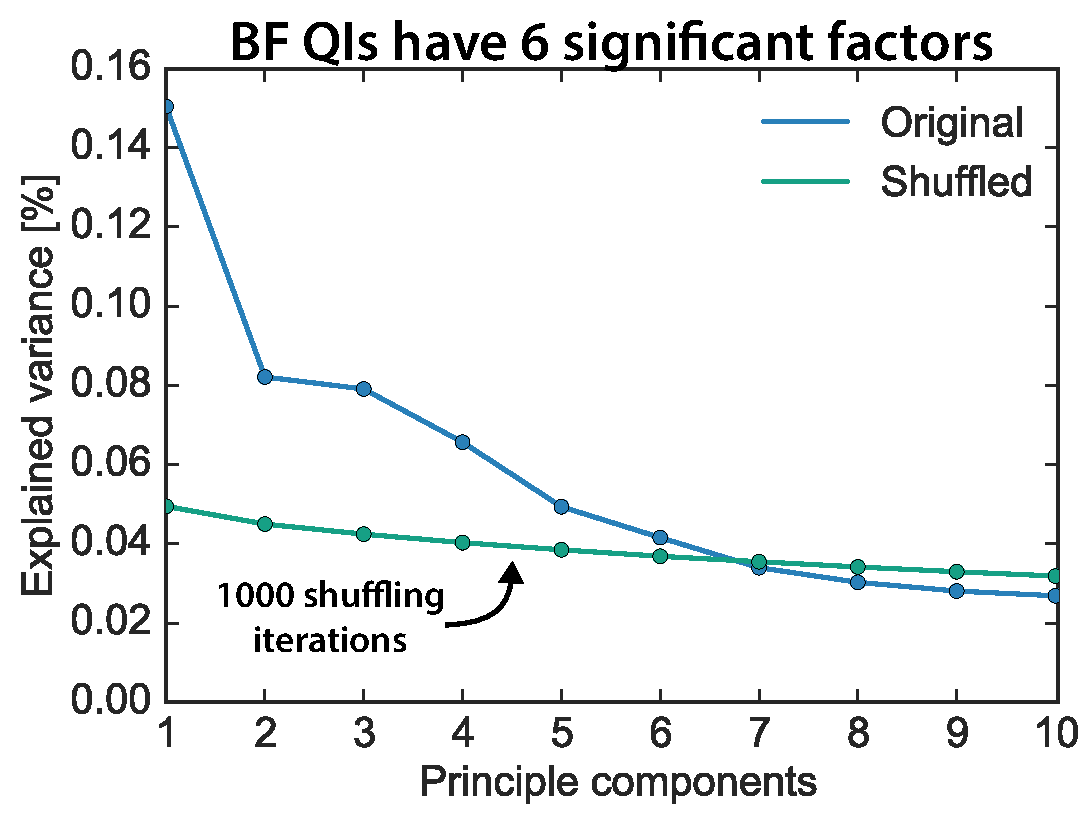
\includegraphics[width=0.95\textwidth]{figures/significantPCs}
	\end{minipage}
	\begin{minipage}[r]{0.49\textwidth}
		\flushright
		\caption{\label{fig:significantPCs}Percentage variance explained of PCs for original and domain shuffled Big Five questionnaire items. The green curve results from 1000 shuffling iterations which are plotted with high transparency. It shows that the six first principle components in Big Five questionnaire item space are significant, because none of the shuffling iteration can produce components of higher explained variance than the first six.}
	\end{minipage}
\end{figure}

\begin{figure}[h!]
	\centering
	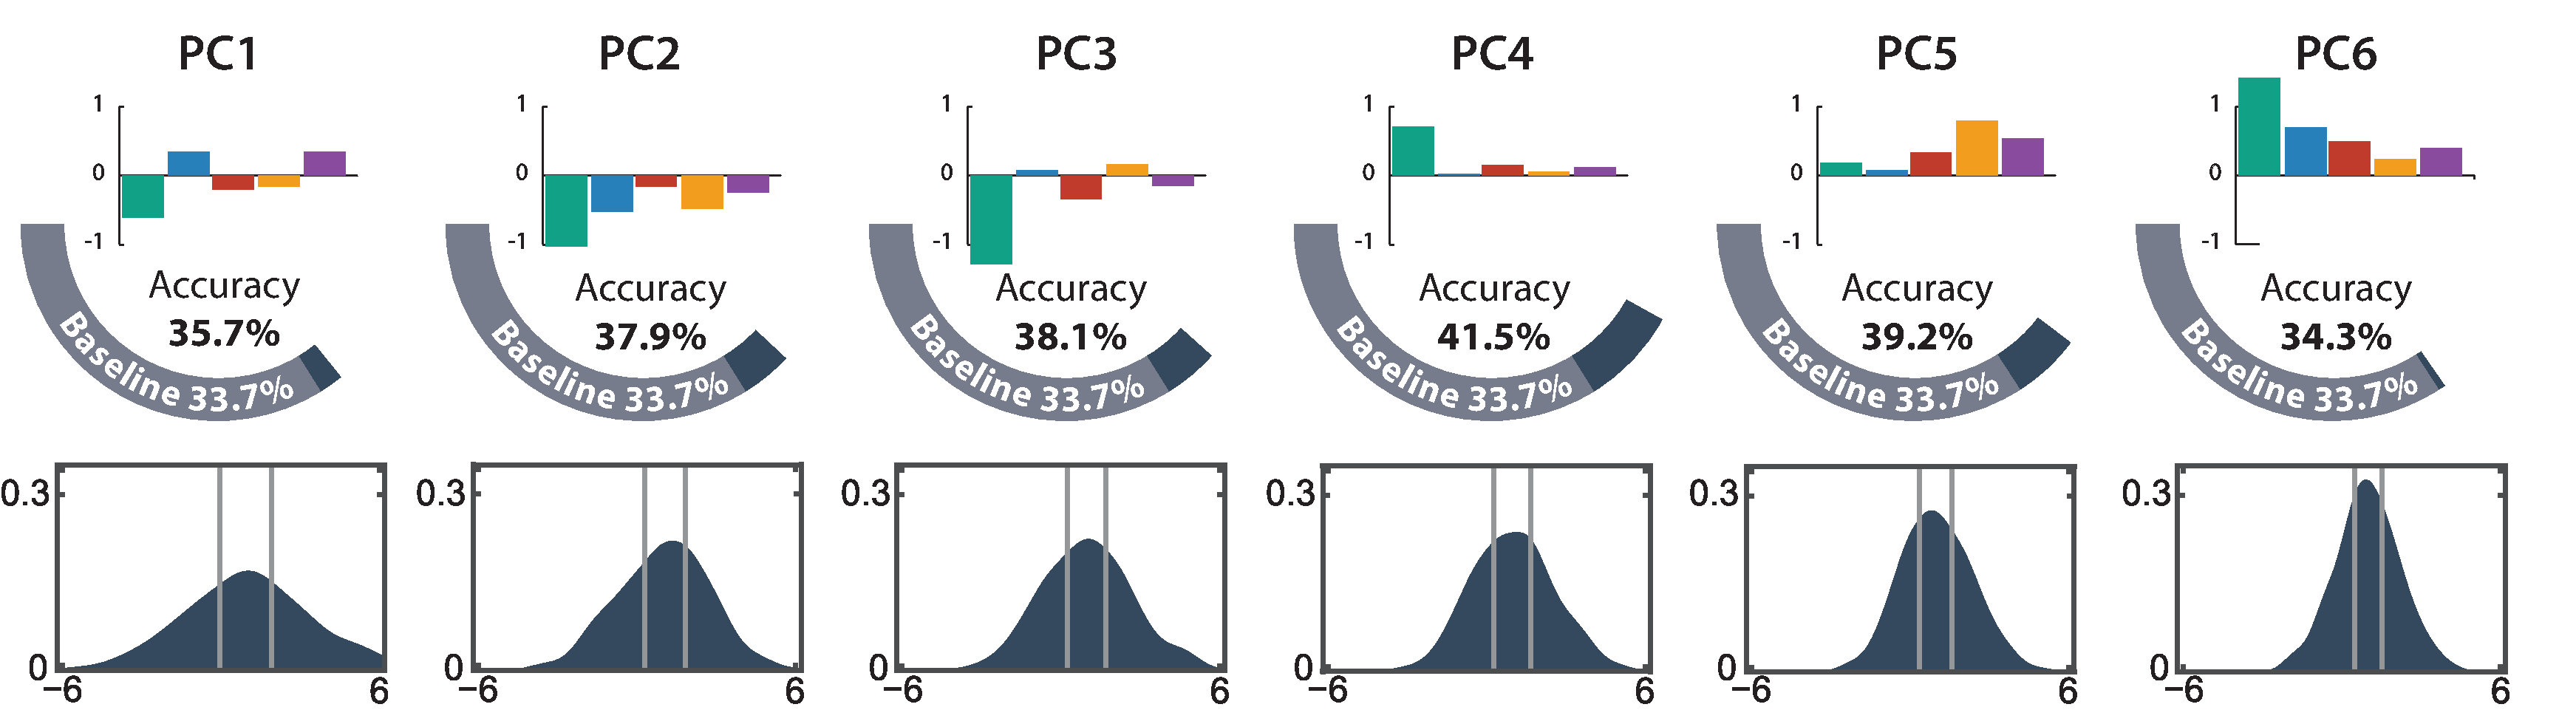
\includegraphics[width=\textwidth]{figures/classification_results_PCA}
	\caption{\label{fig:classification_results_PCA} Three-class classification accuracy of PC components of Big Five Inventory QIs\cite{facet54big}. Same procedure as described in Figure \ref{fig:classification_results_BFT}. The bar diagrams show how each component/archetype is interpreted in terms of BFTs. Bar length correspond to inner products between PC and BF trait.}
\end{figure}
